% ==================================================
% Newton's Forward Difference Expansion
% Discrete Calculus --- Expansions
% ==================================================

\subsection{Newton's Forward Difference Expansion}
\label{sec:newtons-expansion}

\begin{exposition}
In continuous calculus, smooth functions can be expanded as power series
called Taylor series:
\[
f(x)
=
\sum_{k=0}^{\infty} \frac{f^{(k)}(0)}{k!}\, x^k
=
f(0) + f'(0)\,x + \frac{f''(0)}{2!}\,x^2 + \cdots.
\]
The coefficients are determined by successive derivatives evaluated at \(0\),
and the basis functions are ordinary powers \(x^k\).

Discrete calculus has a precise analogue: the \emph{Newton forward difference
expansion}, in which derivatives are replaced by finite differences and
ordinary powers are replaced by falling factorials.
\end{exposition}

\begin{theorembox}{Theorem (Newton Forward Difference Expansion)}
Let \(f : \mathbb{Z} \to \mathbb{R}\). Then \(f\) can be expressed as
\[
f(x)
=
\sum_{k=0}^{n} \frac{\Delta^k f(0)}{k!}\, x^{\underline{k}}
=
f(0)
+
\Delta f(0)\, x
+
\frac{\Delta^2 f(0)}{2!}\, x^{\underline{2}}
+
\frac{\Delta^3 f(0)}{3!}\, x^{\underline{3}}
+
\cdots,
\]
where \(x^{\underline{k}} = x(x-1)\cdots(x-k+1)\) is the falling factorial.
For a polynomial of degree \(n\), the expansion is exact (the series
terminates at \(k = n\)).
\end{theorembox}
\label{thm:newton-expansion}

\begin{remark*}[Standard quantified statement]
\(\forall f : \mathbb{Z}\to\mathbb{R}\) polynomial of degree \(\le n,\;
\forall x \in \mathbb{Z}:\;
f(x) = \displaystyle\sum_{k=0}^{n}\binom{x}{k}\Delta^k f(0)\),
where \(\binom{x}{k} := x^{\underline{k}}/k!\).
\end{remark*}

\subsection*{Structural Parallel with the Taylor Series}

\begin{exposition}
The Newton expansion mirrors the Taylor series at every point. The
correspondence is exact:

\begin{center}
\renewcommand{\arraystretch}{1.5}
\begin{tabular}{|c|c|}
\hline
\textbf{Taylor Series (continuous)} & \textbf{Newton Expansion (discrete)} \\
\hline
Coefficients \(f^{(k)}(0)/k!\) & Coefficients \(\Delta^k f(0)/k!\) \\
Basis functions \(x^k\) & Basis functions \(x^{\underline{k}}\) \\
Derivative \(f^{(k)}\) & Difference \(\Delta^k\) \\
Convergence required in general & Exact for polynomials \\
\hline
\end{tabular}
\end{center}
\end{exposition}

\begin{remark*}[Interpretation]
In the Taylor series, powers \(x^k\) are the natural basis because
the derivative satisfies \(\tfrac{d}{dx}x^k = kx^{k-1}\) and
\(\tfrac{d^m}{dx^m}x^k\big|_{x=0} = k!\) when \(m=k\), and \(0\) otherwise.
The falling factorials satisfy the same two properties under \(\Delta\):
\(\Delta\,x^{\underline{k}} = k\,x^{\underline{k-1}}\) and
\(\Delta^m\,x^{\underline{k}}\big|_{x=0} = k!\) when \(m=k\), else \(0\).
This ``triangular'' property is exactly what allows the coefficients
\(c_k = \Delta^k f(0)/k!\) to be read off independently, level by level.
\end{remark*}

\subsection*{Proof Sketch}

\begin{exposition}
We construct the expansion term by term, matching the values of \(f\) at
successive integers.

The constant term \(f(0)\) matches \(f\) at \(x = 0\).

Adding the linear term \(\Delta f(0)\cdot x\) matches \(f\) at \(x = 0\)
and \(x = 1\).

Adding the quadratic term \(\tfrac{\Delta^2 f(0)}{2!}\,x^{\underline{2}}\)
corrects the value at \(x = 2\) while leaving earlier matches intact,
because \(x^{\underline{2}} = x(x-1)\) vanishes at \(x = 0\) and \(x = 1\).

At each stage, \(x^{\underline{k}}\) vanishes at \(x = 0, 1, \dots, k-1\),
so the \(k\)-th term corrects only the value at \(x = k\). The coefficient
\(\Delta^k f(0)/k!\) achieves this correction by the triangular property
noted above.
\end{exposition}

\subsection*{Reading Coefficients from the Difference Table}

\begin{exposition}
The coefficients in the Newton expansion are read from the \emph{left
edge} of the difference table --- the ``Newton diagonal'':
\[
f(0),\quad
\Delta f(0),\quad
\Delta^2 f(0),\quad
\Delta^3 f(0), \dots
\]

\begin{center}
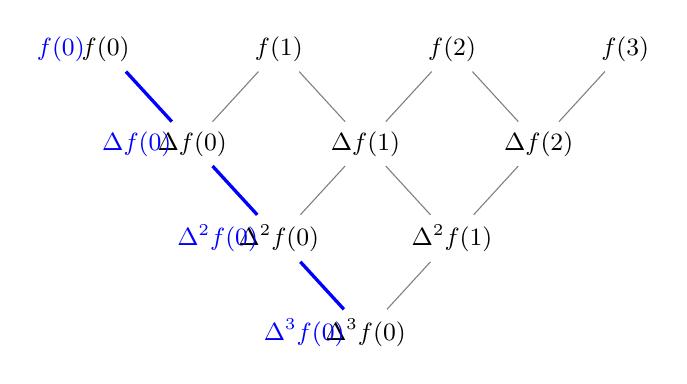
\begin{tikzpicture}[
every node/.style={font=\small},
x=2.2cm,
y=1.2cm
]
\node (f0) at (0,0) {$f(0)$};
\node (f1) at (1,0) {$f(1)$};
\node (f2) at (2,0) {$f(2)$};
\node (f3) at (3,0) {$f(3)$};

\node (d0) at (0.5,-1) {$\Delta f(0)$};
\node (d1) at (1.5,-1) {$\Delta f(1)$};
\node (d2) at (2.5,-1) {$\Delta f(2)$};

\node (d20) at (1,-2) {$\Delta^2 f(0)$};
\node (d21) at (2,-2) {$\Delta^2 f(1)$};

\node (d30) at (1.5,-3) {$\Delta^3 f(0)$};

\draw[gray] (f0)--(d0); \draw[gray] (f1)--(d0);
\draw[gray] (f1)--(d1); \draw[gray] (f2)--(d1);
\draw[gray] (f2)--(d2); \draw[gray] (f3)--(d2);
\draw[gray] (d0)--(d20); \draw[gray] (d1)--(d20);
\draw[gray] (d1)--(d21); \draw[gray] (d2)--(d21);
\draw[gray] (d20)--(d30); \draw[gray] (d21)--(d30);

\draw[very thick,blue] (f0)--(d0)--(d20)--(d30);
\node[blue,left=4pt] at (f0) {$f(0)$};
\node[blue,left=4pt] at (d0) {$\Delta f(0)$};
\node[blue,left=4pt] at (d20) {$\Delta^2 f(0)$};
\node[blue,left=4pt] at (d30) {$\Delta^3 f(0)$};
\end{tikzpicture}

\end{center}

Each level of the difference table contributes exactly one term to the
falling-factorial expansion.
\end{exposition}

\subsection*{\texorpdfstring{Worked Example: Expanding \(f(n) = n^3\)}{Worked Example: Expanding f(n) = n cubed}}

\begin{example*}
We compute the difference table at \(n = 0\):
\[
\begin{array}{c|c|c|c|c}
n & f(n) & \Delta f(n) & \Delta^2 f(n) & \Delta^3 f(n) \\
\hline
0 & 0  & 1  & 6  & 6 \\
1 & 1  & 7  & 12 &   \\
2 & 8  & 19 &    &   \\
3 & 27 &    &    &
\end{array}
\]

The coefficients are \(c_k = \Delta^k f(0)/k!\):
\[
c_0 = 0,\quad c_1 = 1,\quad c_2 = \frac{6}{2} = 3,\quad c_3 = \frac{6}{6} = 1.
\]

Therefore the Newton expansion is:
\[
n^3
= n + 3\,n^{\underline{2}} + n^{\underline{3}}
= n + 3n(n-1) + n(n-1)(n-2).
\]

Verification: \(n + 3n^2 - 3n + n^3 - 3n^2 + 2n = n^3.\) \(\checkmark\)
\end{example*}

\subsection*{\texorpdfstring{Application: Computing \(\sum_{k=0}^{n-1} k^2\)}{Application: Computing sum k=0 to n-1 k squared}}

\begin{example*}
Using the expansion \(k^2 = k^{\underline{1}} + k^{\underline{2}}\) and the
Fundamental Theorem of Finite Calculus (Theorem~\ref{thm:fundamental-theorem-finite-calculus}),

\[
\sum_{k=0}^{n-1} k^2
= \sum_{k=0}^{n-1} k^{\underline{1}} + \sum_{k=0}^{n-1} k^{\underline{2}}.
\]

Since \(\Delta\!\left(\tfrac{k^{\underline{2}}}{2}\right) = k^{\underline{1}}\) and
\(\Delta\!\left(\tfrac{k^{\underline{3}}}{3}\right) = k^{\underline{2}}\),
the Fundamental Theorem gives:
\[
\sum_{k=0}^{n-1} k^{\underline{1}}
= \frac{n^{\underline{2}}}{2} - \frac{0^{\underline{2}}}{2}
= \frac{n(n-1)}{2},
\]
\[
\sum_{k=0}^{n-1} k^{\underline{2}}
= \frac{n^{\underline{3}}}{3} - \frac{0^{\underline{3}}}{3}
= \frac{n(n-1)(n-2)}{3}.
\]

Adding:
\[
\sum_{k=0}^{n-1} k^2
= \frac{n(n-1)}{2} + \frac{n(n-1)(n-2)}{3}
= \frac{n(n-1)}{6}\bigl[3 + 2(n-2)\bigr]
= \frac{n(n-1)(2n-1)}{6}.
\]
\end{example*}

\begin{remark*}[Interpretation]
The standard formula is \(\displaystyle\sum_{k=1}^{n} k^2 = \tfrac{n(n+1)(2n+1)}{6}\).
The computed result \(\displaystyle\sum_{k=0}^{n-1} k^2 = \tfrac{(n-1)n(2n-1)}{6}\) matches:
substitute \(n \mapsto n-1\) in the standard formula to get
\(\tfrac{(n-1)n(2n-1)}{6}\). \(\checkmark\)

This example illustrates the power of the method: the sum was evaluated
by pure algebraic antidifferentiation, with no need for induction or
clever manipulation.
\end{remark*}
